%!TEX root = ../main.tex

\chapter{Introduction}
\label{chp:intro}

\section{Case introduction}

At the university hospital of Padua, 
there is a very important cardiac surgery center where various heart interventions are performed on many people,
the need to teach and visualize the case of operation is very important. \\
Thanks to MRI, doctors can see not only pictures of the heart, but also can even make 3D models.
Each 3D model can show every detail of the patient heart, this can make medics able to analyze and show where and how to resolve the problem.

\subsection{Virtual reality head mounted displays}

The university of Padua has some Meta quest 2\footnote{All rights to meta reserved} [fig:\ref{fig:metaQuest2}] a \ac{HMD} for \ac{VR}. \\
The Meta Quest 2 is a standalone \ac{HMD}, this means that they don't need other peripherals like an external console or \ac{PC} for working.\\
For navigating, the Meta Quest 2 uses two wireless controller, but it also has the possibility to just use your own hands to navigate the interfaces.
For the context awareness it uses 4 infrared cameras and sensors like multi axes gyroscopes and accelerometers.\\
They use a custom version of the Android \ac{OS}, this can give a certain degree of liberty in creating APPs for the device.

\begin{figure}[h]
  \centering
  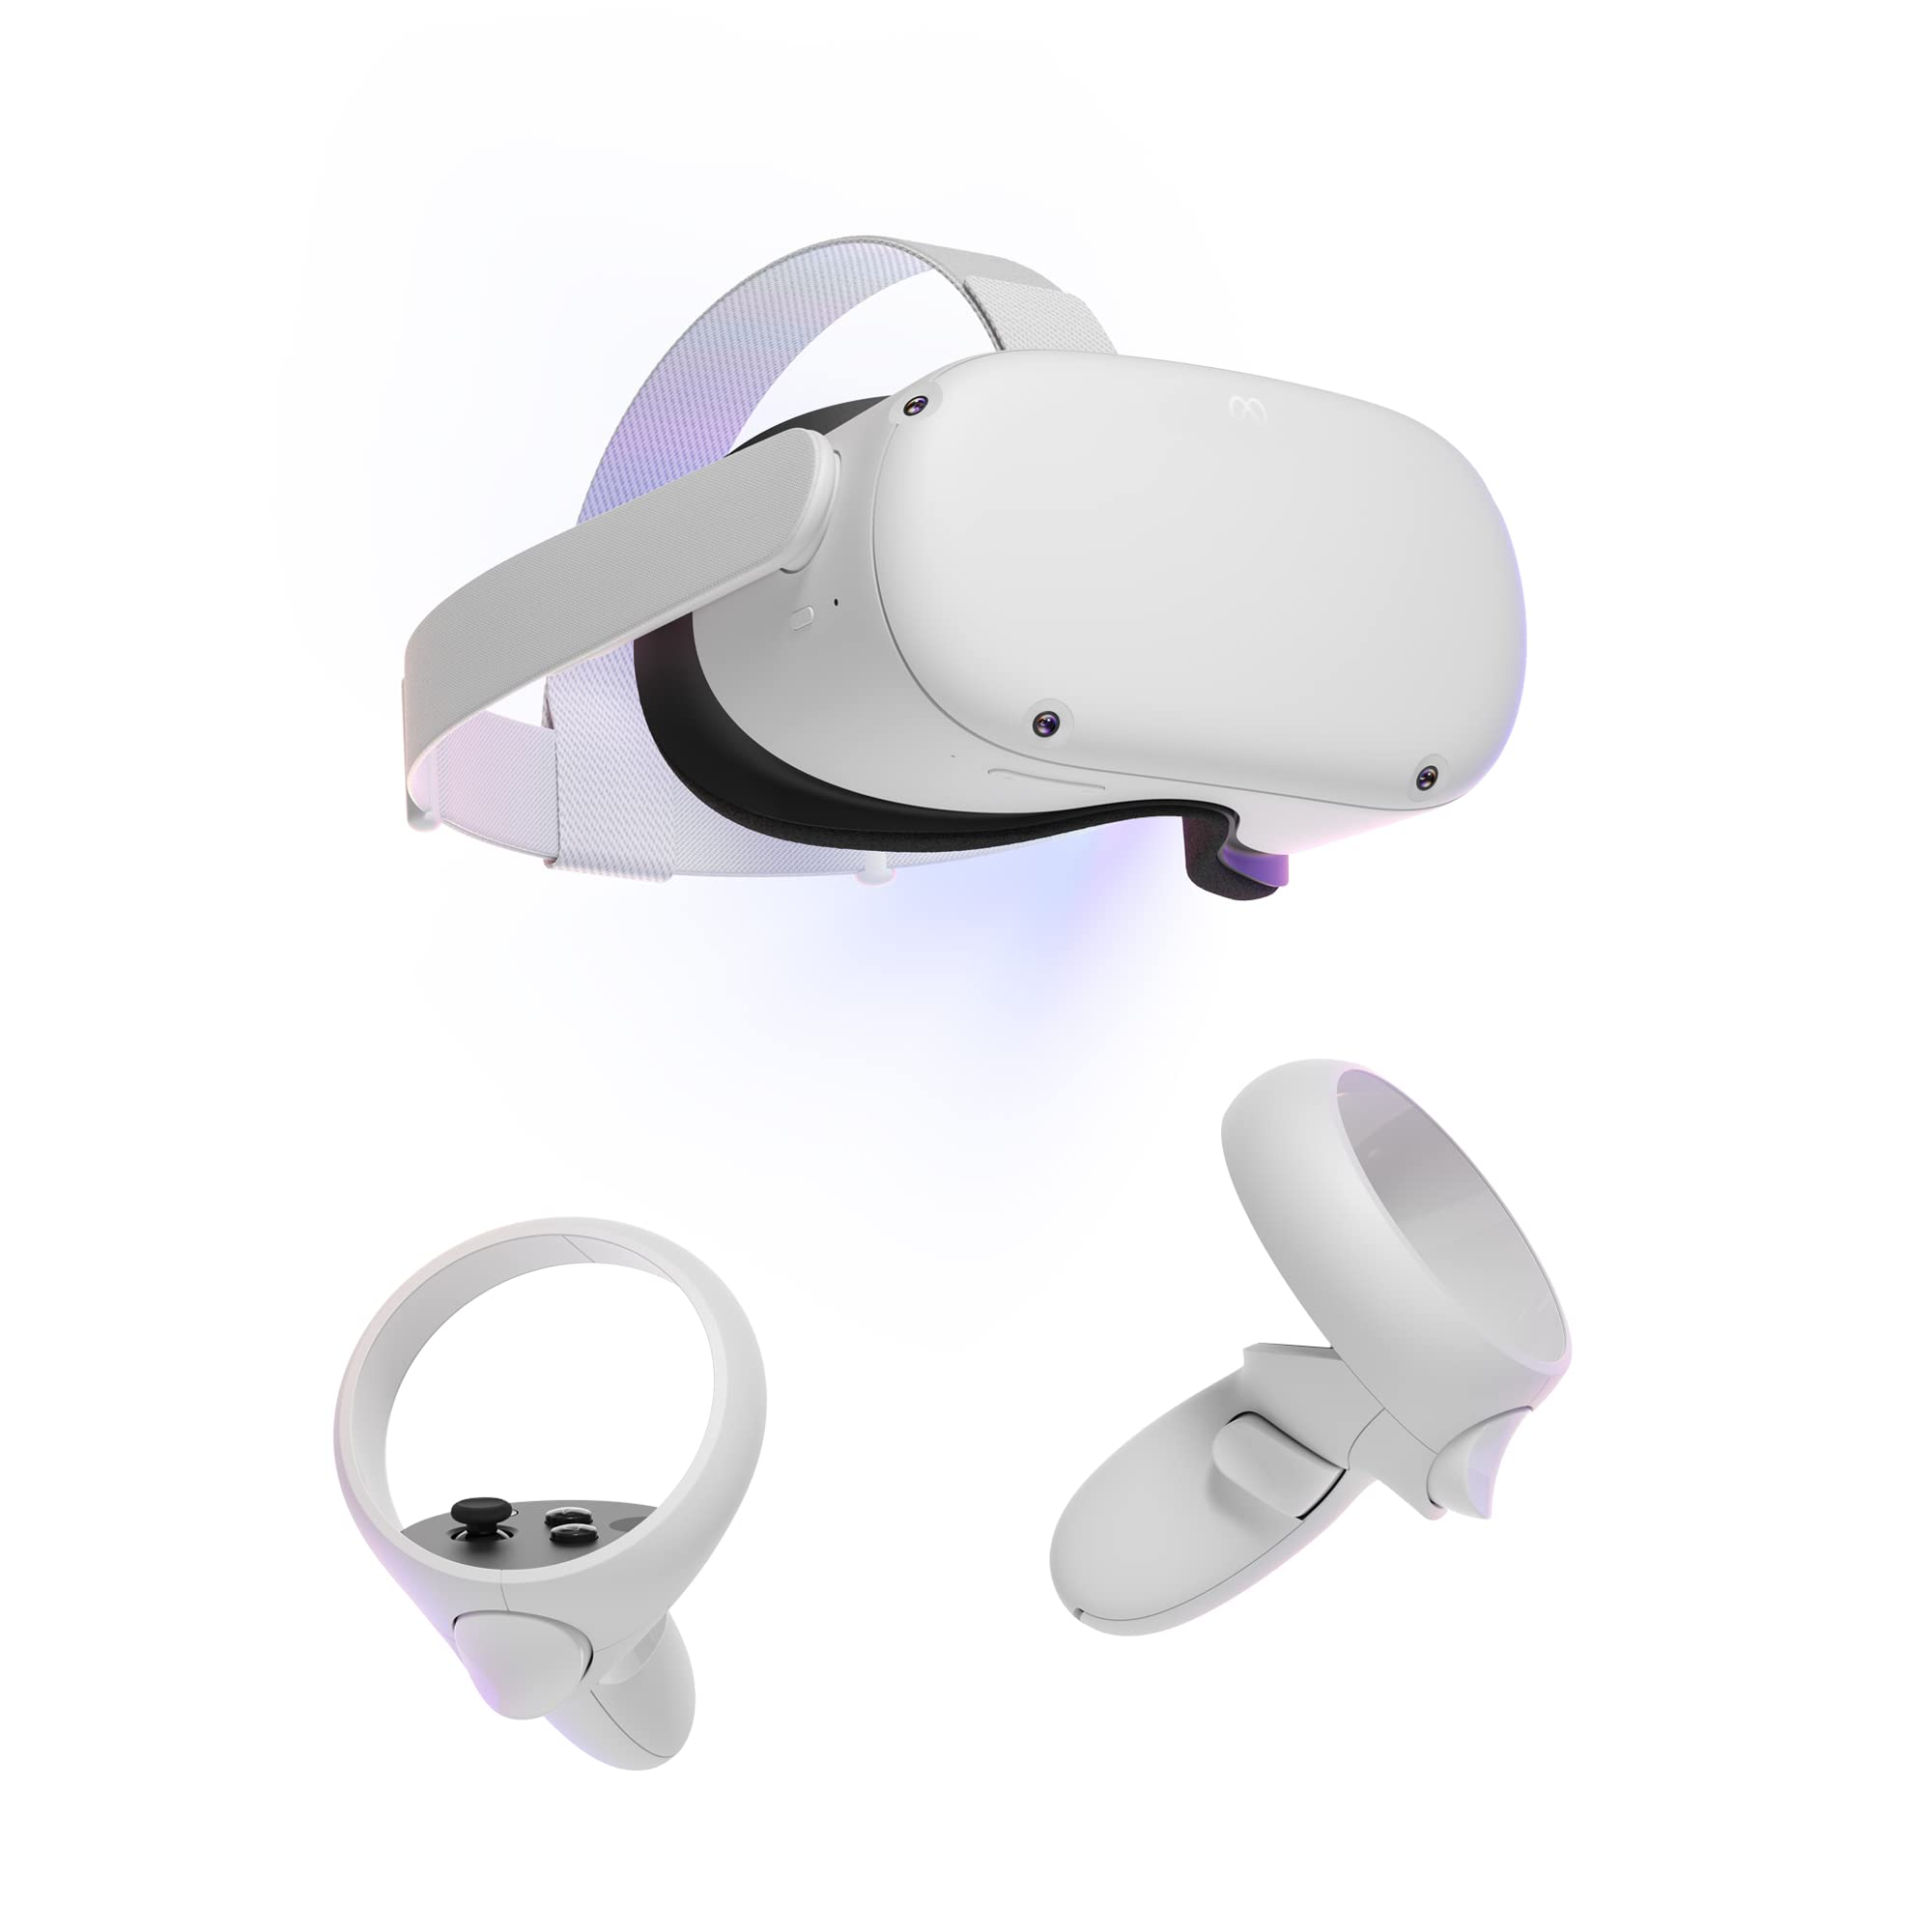
\includegraphics[width=0.5\textwidth]{metaQuest2.jpg}
  \caption{Meta quest 2}
  \label{fig:metaQuest2}
\end{figure}

\subsection{Use cases of VR}
Principally the medics are using VR equipment for training and showing critical health conditions of different patients hearts.
They are using an APP called Shapes XR, this APP has a web interface for upload 3D models and then show them on the \ac{HMD}.
The app has a multiplayer functionality so that multiple people can look at the 3D models in the environment, even if the developers recommend at max 8 people, they tested with 14 users connected and there weren't any problems.

\subsection{APP problems}

Unfortunately Shapes XR is principally used for 3D modelling, so the app has a lot of features like changing the scale of the world or brushes for modelling the objects that aren't useful for the medics,
and quite distracting because for a lot of people is the first time using a \ac{HMD}.\\
The user experience is extremely important in \ac{VR} because is difficult to tutoring the user while is using the \ac{HMD}.
Then Shapes XR position the user in an empty 3D plane with little to none point of reference so If a user accidentally uses the teleport function, they may find themselves somewhere far away from the scene they are supposed to be watching.

\subsubsection{Example of list}
\begin{itemize}
  \item Item 1
  \item Item 2
\end{itemize}

\subsection{A subsection}


\subsubsection{Example of enumeration}
\begin{enumerate}
  \item Item 1
  \item Item 2
\end{enumerate}

\subsubsection{Example of quote}
\begin{displayquote}
Lorem ipsum dolor sit amet, consectetur adipiscing elit, sed do eiusmod tempor incididunt ut labore et dolore magna aliqua.
\end{displayquote}

\paragraph{}
Lorem ipsum dolor sit amet, consectetur adipiscing elit, sed do eiusmod tempor incididunt ut labore et dolore magna aliqua. Ut enim ad minim veniam, quis nostrud exercitation ullamco laboris nisi ut aliquip ex ea commodo consequat. Duis aute irure dolor in reprehenderit in voluptate velit esse cillum dolore eu fugiat nulla pariatur. Excepteur sint occaecat cupidatat non proident, sunt in culpa qui officia deserunt mollit anim id est laborum.